
\refstepcounter{Exercise}
\clearpage\subsection*{\theExercise 赤外線をウェブページから送信する}
\addtocounter{Exercise}{-1}\refstepcounter{Exercise}\label{E:IR}

% \clearpage\subsection*{赤外線をウェブページから送信する}
CGIを使ってウェブページから赤外線を送信できるようにしましょう。

まずは、サンプルを動かしてみましょう。

ウェブブラウザを開いて

localhost:3000/ir.html

を開きましょう。

%
%開いた画像
%
%koyaman
%September 20, 2019 4:01 AM


\centering
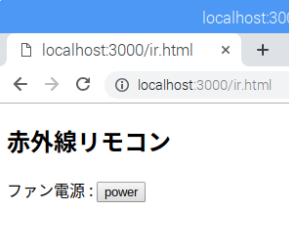
\includegraphics[width=10cm]{text07-img/ome7-img061.png}
\flushleft

ボタンを押すとCGIで赤外線の送信をするコマンドが実行されます。

コマンドは、

irsend SEND\_ONCE fan onoff

が実行されます。リモコンの名前はfan、信号の名前はonoffになっています。

リモコンの名前、信号の名前が違う場合は、

{\textasciitilde}/07/www/cgi-bin/ir.hsp

を開いて

exec “irsend SEND\_ONCE fan onoff”

を変更して保存しましょう。

同じ場合はそのままで\ruby{大丈夫}{だいじょうぶ}です。

%
%スクショ
%ir.htmlのボタン
%koyaman
%September 20, 2019 4:05 AM


\centering
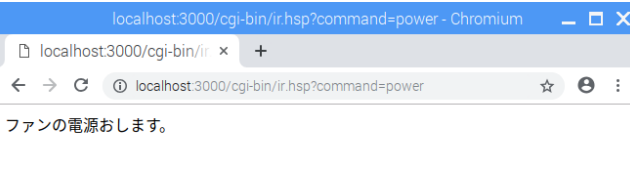
\includegraphics[width=10cm]{text07-img/ome7-img062.png}
\flushleft

ブラウザのファン\ruby{電源}{でんげん}ボタンを押すと、CGIが起動して

赤外線を送信します。


\bigskip

\clearpage
プログラム解説

{\textasciitilde}/07/www/ir.html

8行目でフォームの\ruby{内容}{ないよう}を受け取るCGIを設定しています。


\begin{table}[htbp]
    \centering
    % \caption{文字タイプ表}
    \begin{tabular}{|l|}
        \hline
        
        1. {\textless}!DOCTYPE html{\textgreater}\\ 
        2. {\textless}html{\textgreater}\\
        3. {\textless}head{\textgreater}
        4. \ \ \ \ {\textless}meta charset={\textquotedbl}utf-8{\textquotedbl}{\textgreater}\\
        5. {\textless}/head{\textgreater}\\
        6. {\textless}body{\textgreater}\\
        7. \ \ \ \ {\textless}h2{\textgreater}赤外線リモコン{\textless}/h2{\textgreater}\\
        8. \ \ \ \ {\textless}form action={\textquotedbl}cgi-bin/ir.hsp{\textquotedbl} method={\textquotedbl}GET{\textquotedbl}{\textgreater}\\
        9. \ \ \ \ \ \ \ \ {\textless}p{\textgreater}\\
        10. \ \ \ \ \ \ \ \ \ \ \ \ ファン電源 : {\textless}input type={\textquotedbl}submit{\textquotedbl} value={\textquotedbl}power{\textquotedbl} name={\textquotedbl}command{\textquotedbl}{\textgreater}\\
        11. \ \ \ \ \ \ \ \ {\textless}/p{\textgreater}\\
        12. \ \ \ \ {\textless}/form{\textgreater}\\
        13. {\textless}/body{\textgreater}\\
        14. {\textless}/html{\textgreater}\\
        \hline
    \end{tabular}
\end{table}



{\textasciitilde}/07/www/cgi-bin/ir.hsp

がCGIとしてに起動します。

10行目で送信ボタンを作っています。

{\textless}input type={\textquotedbl}submit{\textquotedbl} value={\textquotedbl}power{\textquotedbl}
name={\textquotedbl}command{\textquotedbl}{\textgreater}

クエリストリングの名前はcommandで値はpowerとなります。このボタンが押されるとCGIが起動します。

\clearpage
\bigskip


\bigskip

\bigskip





\begin{table}[htbp]
    \centering
    % \caption{文字タイプ表}
    \begin{tabular}{|l|}
        \hline
        
        1. \#include {\textquotedbl}hsp3cl.as{\textquotedbl}\\ 
        2. \#include {\textquotedbl}cmdexec.as{\textquotedbl}\\
        3. \#include {\textquotedbl}cgi.as{\textquotedbl}
        4. \\
        5. mes {\textquotedbl}Content-type: text/html{\textbackslash}n{\textquotedbl}\\
        6. mes {\textquotedbl}{\textless}html{\textgreater}{\textless}head{\textgreater}{\textless}meta charset={\textbackslash}{\textquotedbl}utf-8{\textbackslash}{\textquotedbl}{\textgreater}{\textless}/head{\textgreater}{\textless}body{\textgreater}{\textquotedbl}\\
        7. \\
        8. getqueryval {\textquotedbl}command{\textquotedbl}, cmd\\
        9. if cmd = {\textquotedbl}power{\textquotedbl} \{\\
        10. \ \ mes {\textquotedbl}{\textless}p{\textgreater}ファンの電源をおします。{\textless}/p{\textgreater}{\textquotedbl}\\
        11. \ \ exec {\textquotedbl}irsend SEND\_ONCE fan onoff{\textquotedbl}\\
        12. \} else \{\\
        13. \ \ \ \ mes {\textquotedbl}{\textless}p{\textgreater}コマンドが正しくありません{\textless}/p{\textgreater}{\textquotedbl}\\
        14. \ \ \ \ mes {\textquotedbl}{\textless}p{\textgreater}{\textquotedbl} + cmd + {\textquotedbl}{\textless}/p{\textgreater}{\textquotedbl}\\
        15. \}\\
        16. \\
        17. mes {\textquotedbl}{\textless}/body{\textgreater}{\textless}/html{\textgreater}{\textquotedbl}\\
        18. end\\
        \hline
    \end{tabular}
\end{table}

\bigskip


\bigskip


\bigskip

8行目でクエリストリングから名前がcommandに対応する値を取り出してcmd変数へ入れています。

9〜15行目で受け取ったcmd変数をもとに条件判断をしています。cmdがpowerのときにファンの電源をつける赤外線を送っています。

それ以外の場合は正しいコマンドでないとして、メッセージを表示しています。


\bigskip

\bigskip
\refstepcounter{Question}\theQuestion\label{Q:IR}

% 問題7-15  
% ファンの電源をつける以外の赤外線送信機能を追加してみよう。

\ \ HINT :
まずは、ir.htmlにボタンを追加しよう。

\ \ \ \ そのあと、ir.hspの条件判断を追加しよう。

ir.htmlのフォームを自己紹介ページの一番下に付け加えよう。


\bigskip


\bigskip


\clearpage
\label{P:gpio}
CGIを使うときに便利なHSPの命令一覧



\begin{table}[htbp]
    \centering
    % \caption{文字タイプ表}
    \begin{tabular}{|l|l|l|}
        \hline
        \begin{tabular}{l}
            命令名/使い方
        \end{tabular}
        &
        \begin{tabular}{l}
            例題
        \end{tabular}
        &
        \begin{tabular}{l}
            効果
        \end{tabular}
        \\\hline


        %1行目
        \begin{tabular}{l}
            \#include “cgi.as” \\
            getqueryval “name”, var 
        \end{tabular}
        &
        \begin{tabular}{l}
            例題 7-8\\
            例題 7-9\\
            例題 7-10\\
            例題 7-11
        \end{tabular}
        &
        \begin{tabular}{l}
            クエリストリングから名前”name”を探し\\
            て文字列として値を変数varへ入れる。\\
		    \textbf{localhost:3000/cgi-}\\
            \textbf{bin/querystring.hsp?name=val}\\
		    の場合、varにはvalが入る。
        \end{tabular}
        \\\hline


        %2行目
        \begin{tabular}{l}
            \#include “rpz-gpio-cl.as”\\
            onoff = cgpioin(17)
        \end{tabular}
        &
        \begin{tabular}{l}
            例題 7-7\\
            例題 7-9\\
            例題 7-11
        \end{tabular}
        &
        \begin{tabular}{l}
            gpio 命令と使い方は同じ。GPIO17 番に 1 \\
            を書き込む。gpio 命令との違いはプログラ\\
            ム終了時にも書き込んだ値が持続する。例\\
            えば、cgpio 17, 1 を実行すると、プログラ\\
            ム終了時でも 17 番の GPIO は 1 のままに\\
            なる。
        \end{tabular}
        \\\hline


        %3行目
        \begin{tabular}{l}
            \#include “rpz-gpio-cl.as”\\
		    onoff = cgpioin(17)
        \end{tabular}
        &
        \begin{tabular}{l}
            例題 7-7
        \end{tabular}
        &
        \begin{tabular}{l}
            gpio 命令と同じ。cgpio でプログラム終了\\
            時でも効果を持続させたい場合はこちらを\\
            使用する必要がある。
        \end{tabular}
        \\\hline


        %4行目
        \begin{tabular}{l}
            \#include “rpz-gpio-cl.as”
        \end{tabular}
        &
        \begin{tabular}{l}
            例題 7-7\\
            例題 7-9\\
            例題 7-11
        \end{tabular}
        &
        \begin{tabular}{l}
            \#include “rpz-gpio.as”のコマンドライン\ruby{版}{ばん}\\
		    コマンドラインや CGI で動くプログラムを書\\
		    く場合はこちらを使う。cgpio, cgpioin 命令\\
		    以外は同じ命令が使える。
        \end{tabular}
        \\\hline


        %5行目
        \begin{tabular}{l}
            \#include “jtalk.as”\\
            jtsave “こんにちは”, hello 
        \end{tabular}
        &
        \begin{tabular}{l}
            例題 7-10
        \end{tabular}
        &
        \begin{tabular}{l}
            “こんにちは”をOpenJtalkで音声合成を\\
            して、作った音声ファイルのファイル名を\\
            hello変数へ入れる。音声ファイルは/tmp/\\
            ディレクトリの下にランダムなファイル名\\
            で入る。\\
            例えば、hello変数の中身は\\		
            “/tmp/tmp.abzgda”のような感じになる。 
        \end{tabular}
        \\\hline

        %6行目
        \begin{tabular}{l}
            end
        \end{tabular}
        &
        \begin{tabular}{l}
            すべての例題
        \end{tabular}
        &
        \begin{tabular}{l}
            プログラムの終了を意味する。この命令は\\
            CGI用のプログラムを終了するときに必要。\\
            この命令がないとCGIのプログラムは終了\\
            しない。(ブラウザの読み込みが終わらなく\\
            なる。)
        \end{tabular}
        \\\hline
        
        
    \end{tabular}
    \end{table}







\bigskip

{\bfseries
	付録 ウェブサーバの停止方法}

電源を切る前、ウェブサーバが起動しているターミナルを\ruby{閉}{と}じる前、ウェブサーバを停止したいときは、ウェブサーバを起動したターミナル(./webserver.pyを実行している画面)を選択して


\bigskip

CtrlとCを同時に押します。


\bigskip

それでウェブサーバは終了します。


\bigskip


\bigskip


\bigskip
